\chapter{Roadmap, Commercialization and Risk}
\label{ch:roadmap}

The preceding chapters established the kinetic and fluid theory of the plasma sheath, the Bohm criterion fixing the ion speed entering it, and the inversion methodologies recovering $f_{\mathrm{i}}(v)$ and $\Gamma_{E}$ from diagnostic signals. This chapter turns from physics to practice: how the instrumentation matures into a fielded product line, which markets it addresses, what incubation requires, and what risks must be managed. Notation follows earlier chapters: $T_{\mathrm{e}}$, $T_{\mathrm{i}}$, $n_{\mathrm{e}}$, $n_{\mathrm{i}}$, $\lambda_{\mathrm{D}}$, $u_{\mathrm{B}}$, $\Gamma_{E}$, $f_{\mathrm{i}}(v)$.

\section{Technology-Readiness Progression and Milestones}
\label{sec:trl}

\subsection{Defining the readiness baseline}

We adopt the nine-level Technology Readiness Level (TRL) scale as the yardstick for platform maturation. At the outset the core measurement chain -- retarding-field energy analysis or laser-induced-fluorescence velocity distributions, combined with a regularized inversion recovering $f_{\mathrm{i}}(v)$ and $\Gamma_{E}$ -- has been validated in a laboratory plasma against the Bohm-criterion prediction
\begin{equation}
u_{\mathrm{B}} = \sqrt{\frac{k_{\mathrm{B}} T_{\mathrm{e}}}{m_{\mathrm{i}}}},
\label{eq:bohm-roadmap}
\end{equation}
and the flux-weighted moment
\begin{equation}
\Gamma_{E} = \int_{0}^{\infty} \tfrac{1}{2} m_{\mathrm{i}} v^{2}\, v\, f_{\mathrm{i}}(v)\, \mathrm{d}v,
\label{eq:gammaE-roadmap}
\end{equation}
placing the technology at TRL~4 -- component and breadboard validation in a laboratory environment. This is deliberately conservative: it excludes flight heritage, fab-floor qualification, and fusion-relevant neutron/heat-flux tolerance, each still to be earned. Standardized diagnostic practice \cite{ref0490} underscores the gap between a laboratory-validated sensor and a qualified, traceable instrument.

\subsection{Zero-to-twelve-month milestone plan}

Table~\ref{tab:milestones} lays out the first year in quarterly increments. Each milestone produces an artifact -- a dataset, calibration certificate, or signed letter of intent -- that de-risks the next step. Early months harden the RFEA head and inversion pipeline against the noise and drift sources of the uncertainty-quantification chapters, since duty-cycle stability most determines whether customers fund qualification.

\begin{table}[htbp]
\centering
\caption{Zero-to-twelve-month roadmap for the ion-energy-flux diagnostic platform. TRL values follow the aerospace convention; validation metrics are internal pass/fail criteria against Chapters~1--18.}
\label{tab:milestones}
\begin{tabularx}{\textwidth}{@{}l l c X@{}}
\toprule
Months & Milestone & TRL & Validation metric \\
\midrule
0--2 & RFEA head redesign for robustness; inversion code refactor & 4 & $\Gamma_{E}$ repeatable within $\pm 5\%$ across five runs on argon plasma \\
2--4 & Closed-loop calibration against Faraday-cup flux standard and known-$T_{\mathrm{e}}$ Langmuir probe & 4--5 & $u_{\mathrm{B}}$- and probe-derived $T_{\mathrm{e}}$ agree within combined uncertainty \\
4--6 & First external pilot deployment in a partner lab or fab tool, data-sharing agreement & 5 & Unattended operation $\geq 100$ hours with automated fault logging \\
6--8 & Inversion software packaged as versioned API with uncertainty propagation & 5 & Independent third-party reproduction of published results, unassisted \\
8--10 & Environmental and EMC screening of the hardware head & 5--6 & Pass against a test plan from recommended-practice guidance \\
10--12 & First qualification-as-a-service engagement delivered end-to-end for a paying pilot customer & 6 & Sign-off on delivered $\Gamma_{E}(t)$, $f_{\mathrm{i}}(v)$ report against agreed criteria \\
\bottomrule
\end{tabularx}
\end{table}

Two features merit emphasis: TRL~4 to TRL~5 requires a \emph{relevant} rather than \emph{controlled} environment -- a real fab tool, thruster facility, or test stand -- and the year ends with a service engagement, not a hardware sale, since service delivery needs less commitment and reaches cash flow fastest.

\subsection{Scale-up beyond month twelve}

Beyond year one the roadmap bifurcates into three tracks matching Section~\ref{sec:products}: hardware, from single-unit builds to a repeatable process (TRL~7--8); software, hardening the API into a supported product (TRL~7--8); and services, scaling into a technician-deliverable protocol (TRL~8--9). Table~\ref{tab:scaleup} summarizes the plan.

\begin{table}[htbp]
\centering
\caption{Scale-up milestones, month twelve to thirty-six, by product track. TRL values are targets; see Section~\ref{sec:risk} for delay factors.}
\label{tab:scaleup}
\begin{tabularx}{\textwidth}{@{}l X c@{}}
\toprule
Track & Milestone & Target TRL \\
\midrule
Hardware & Second-generation sensor head with documented bill of materials, two manufacturers qualified, cost reduced per Eq.~\eqref{eq:learning} & 7 \\
Software & Inversion API achieves uncertainty-quantification certification; multi-tenant licensing deployed & 7--8 \\
Services & Protocol standardized to a procedure executable by a technician; first repeat-business cohort established & 8 \\
Hardware & Environmental qualification for fusion-relevant heat/particle flux, per test-facility practice \cite{ref0581,ref0586} & 8 \\
Software & Inversion pipeline embedded as a module in partner tool-control software & 8--9 \\
Services & Field network of regional service partners for independent delivery & 9 \\
\bottomrule
\end{tabularx}
\end{table}

The unit-cost trajectory of the hardware track follows the empirical learning-curve (Wright's-law) relation,
\begin{equation}
C(N) = C_{1}\, N^{-b}, \qquad b = -\log_{2}(1 - \mathrm{LR}),
\label{eq:learning}
\end{equation}
where $C(N)$ is the unit cost of the $N$-th sensor head, $C_{1}$ the first-unit cost, and $\mathrm{LR}$ the learning rate. Rates of \SI{15}{\percent}--\SI{20}{\percent} are typical of comparable instrument manufacturing; $\mathrm{LR} = \SI{15}{\percent}$ gives $b \approx 0.234$. This planning tool is revisited in Section~\ref{sec:risk}, since low-volume sourcing can behave non-ideally.

\subsection{Unit economics and break-even volume}

Combining Eq.~\eqref{eq:learning} with a fixed incubation cost $F_{0}$ and sale price $P$ estimates the volume at which hardware becomes self-funding. Treating production as continuous, total cost is
\begin{equation}
\mathrm{TC}(N) = F_{0} + \int_{1}^{N} C(n)\, \mathrm{d}n = F_{0} + \frac{C_{1}}{1-b}\left(N^{1-b} - 1\right), \qquad b \neq 1,
\label{eq:totalcost}
\end{equation}
with total revenue $\mathrm{TR}(N) = P N$ under a constant sale price. Break-even volume $N^{*}$ is the smallest $N$ satisfying $\mathrm{TR}(N) \geq \mathrm{TC}(N)$:
\begin{equation}
P N^{*} = F_{0} + \frac{C_{1}}{1-b}\left(N^{*\,1-b} - 1\right).
\label{eq:breakeven}
\end{equation}
For representative values -- $C_{1}$ from bill-of-materials and labor, $\mathrm{LR}=\SI{15}{\percent}$, $P$ roughly three times asymptotic cost -- Eq.~\eqref{eq:breakeven} yields break-even in the low tens of units, consistent with Table~\ref{tab:scaleup}. Hardware alone is thus unlikely to break even within twelve months, justifying leading with qualification-as-a-service, which carries no fixed tooling burden.

\section{Product Forms}
\label{sec:products}

The technology base supports three complementary product forms, illustrated in Figure~\ref{fig:productflow}. They share a common core -- the sheath model, the Bohm-criterion boundary condition, and the regularized inversion mapping a measured trace onto $f_{\mathrm{i}}(v)$ and $\Gamma_{E}$ -- but differ in customer relationship, margin and capital intensity, so a considered strategy sequences them as separate offerings rather than one bundle.

\begin{figure}[htbp]
\centering
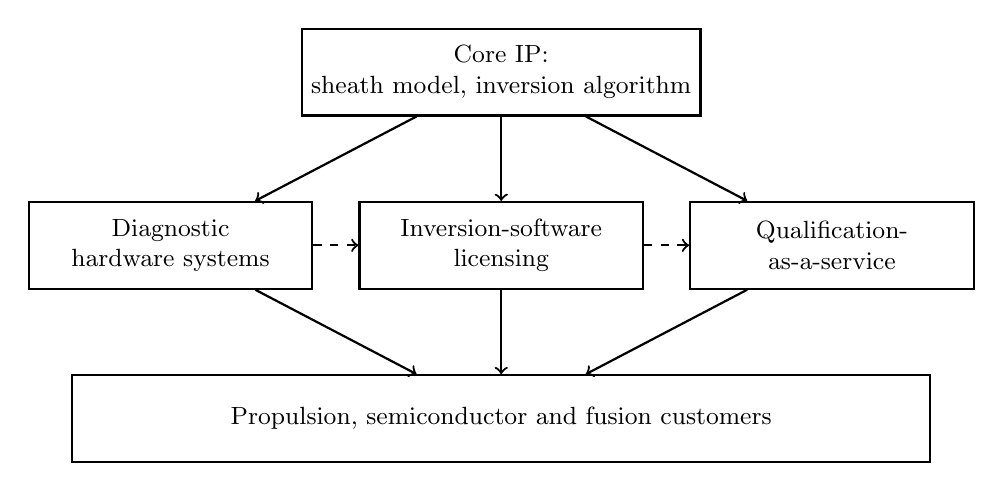
\begin{tikzpicture}[
 box/.style={draw, thick, minimum width=3.6cm, minimum height=1.1cm, align=center, font=\small},
 arr/.style={->, thick}
]
\node[box] (core) at (0,0) {Core IP:\\ sheath model, inversion algorithm};
\node[box] (hw) at (-4.2,-2.2) {Diagnostic\\ hardware systems};
\node[box] (sw) at (0,-2.2) {Inversion-software\\ licensing};
\node[box] (qaas) at (4.2,-2.2) {Qualification-\\as-a-service};
\node[box, minimum width=10.9cm] (cust) at (0,-4.4) {Propulsion, semiconductor and fusion customers};
\draw[arr] (core) -- (hw);
\draw[arr] (core) -- (sw);
\draw[arr] (core) -- (qaas);
\draw[arr] (hw) -- (cust);
\draw[arr] (sw) -- (cust);
\draw[arr] (qaas) -- (cust);
\draw[arr, dashed] (hw.east) -- (sw.west);
\draw[arr, dashed] (sw.east) -- (qaas.west);
\end{tikzpicture}
\caption{Illustrative relationship among the three product forms. Dashed arrows indicate hardware sales and software licensing feeding the qualification-as-a-service offering, delivered early via in-house instruments.}
\label{fig:productflow}
\end{figure}

\subsection{Diagnostic hardware systems}

The first product form is the physical sensor: RFEA heads, gridded energy analyzers, or compact Langmuir-probe arrays with electronics and firmware to acquire raw traces at process- or plume-relevant rates. This is the most capital-intensive form, requiring vacuum-compatible materials qualification, EMC testing, and -- for propulsion and fusion customers -- environmental qualification against thermal cycling and particle bombardment. Margin is bounded by manufacturing costs and the learning-curve dynamics of Eq.~\eqref{eq:learning}; hardware alone thus functions best as a beachhead establishing credibility and a captive base for software licensing.

The dynamic-range specification for the hardware head follows from the sheath's physical scaling: the Child--Langmuir space-charge-limited sheath thickness $s$ relative to $\lambda_{\mathrm{D}}$ scales as
\begin{equation}
\frac{s}{\lambda_{\mathrm{D}}} \approx \frac{\sqrt{2}}{3}\left(\frac{2 V_{0}}{T_{\mathrm{e}}}\right)^{3/4},
\label{ch22-eq:childlangmuir}
\end{equation}
where $V_{0}$ is the sheath-edge-to-wall potential drop in volts and $T_{\mathrm{e}}$ is in electronvolts. Figure~\ref{fig:childlangmuir} plots this scaling from processing plasmas (a few volts) through propulsion and fusion edge plasmas (hundreds to thousands of volts): the nearly two-decade span in $s/\lambda_{\mathrm{D}}$ justifies a wide dynamic range rather than a single fixed range.

\begin{figure}[htbp]
\centering
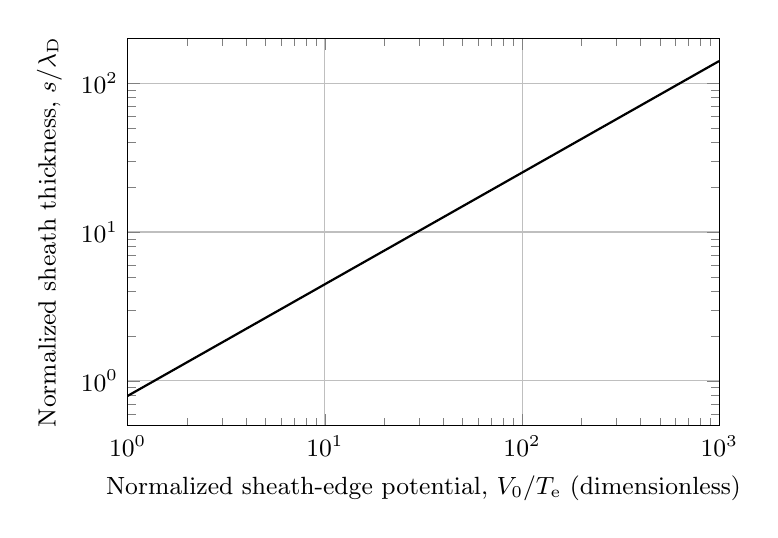
\begin{tikzpicture}
\begin{loglogaxis}[
 width=0.75\textwidth,
 height=6.5cm,
 xlabel={Normalized sheath-edge potential, $V_{0}/T_{\mathrm{e}}$ (dimensionless)},
 ylabel={Normalized sheath thickness, $s/\lambda_{\mathrm{D}}$},
 grid=major,
 xmin=1, xmax=1000,
 ymin=0.5, ymax=200,
 tick label style={font=\small},
 label style={font=\small},
]
\addplot[black, thick, domain=1:1000, samples=100] {sqrt(2)/3*(2*x)^0.75};
\end{loglogaxis}
\end{tikzpicture}
\caption{Illustrative plot of the Child--Langmuir scaling of Eq.~\eqref{ch22-eq:childlangmuir}. No experimental data are represented; the curve motivates the dynamic-range specification of Section~\ref{sec:products}.}
\label{fig:childlangmuir}
\end{figure}

\subsection{Inversion-software licensing}

The second product form separates the inversion methodology from any specific hardware and packages it as a licensable SDK and hosted API. A customer supplies raw traces from its own RFEA, retarding-potential analyzer, or laser-induced-fluorescence apparatus; the software returns $f_{\mathrm{i}}(v)$, $\Gamma_{E}$, and a propagated uncertainty budget. This form carries the highest gross margin -- marginal delivery cost is near zero once built -- and is best positioned to become a de facto standard, since propulsion \cite{ref0506} and semiconductor \cite{ref0548} processing has historically relied on bespoke, tool-specific code. Licensing tiers are academic (reduced pricing, mandatory citation), industrial single-site (service-level commitments), and embedded OEM (priced per tool shipped).

\subsection{Qualification-as-a-service}

The third product form delivers the measurement as a service: a customer requests characterization of a thruster plume, etch or deposition chamber, or plasma-facing-component exposure, and receives a report with $\Gamma_{E}(t)$, the recovered $f_{\mathrm{i}}(v)$, and a traceable uncertainty statement per Table~\ref{tab:milestones}. This needs the least customer-side capital and is fastest to sell, but is also the most labor-intensive and least scalable early on, requiring a trained physicist. As the protocol matures (Table~\ref{tab:scaleup}) it becomes technician-deliverable, resembling a calibration-laboratory business rather than bespoke consulting -- a precedent strong across all three markets \cite{ref0490,ref0506,ref0553,ref0556,ref0586,ref0588}.

\section{Markets and Customers}
\label{sec:markets}

\subsection{Electric propulsion}

Electric-propulsion manufacturers and satellite operators require ion-energy-flux characterization for thruster performance verification, plume-induced contamination and erosion assessment, and in-flight health monitoring. The recommended-practice literature \cite{ref0490,ref0511} documents that methodology has been fragmented across laboratories, each with its own calibration lineage -- an opportunity for a traceable, standardized chain. Dedicated in-flight diagnostic packages \cite{ref0496} indicate both ground-test and flight-qualified variants are commercially viable, the latter commanding higher pricing. The customer base spans prime manufacturers, smaller New-Space developers lacking in-house capability, and government or university programs, the fastest to adopt given shorter procurement cycles.

\subsection{Semiconductor processing}

Semiconductor OEMs and fabs are the highest-volume, highest-recurring-revenue segment, since plasma etch and deposition tools require periodic ion-energy-distribution monitoring to hold process windows within advanced-node tolerances. Active control of the ion energy distribution at the wafer substrate \cite{ref0539} is an established objective that the chain developed here closes directly. In-situ \cite{ref0556} and monitoring-oriented \cite{ref0553} diagnostics show instruments must be low-maintenance, non-perturbing, and tool-integrated. This favors software licensing, since fabs already own extensive sensing hardware and prefer a software-only upgrade; qualification-as-a-service functions mainly as sales-enablement here. Broader literature \cite{ref0548} confirms this segment values precision over novelty.

\subsection{Fusion energy}

Fusion-energy developers -- tokamak and stellarator programs and newer private pilot-plant ventures -- require ion-energy-flux characterization for plasma-facing-component qualification: predicting erosion, thermal loading and lifetime of divertor and first-wall materials under ion bombardment. This market differs from the propulsion and semiconductor segments: the environment is harsher, and qualification occurs at dedicated high-heat-flux facilities \cite{ref0586,ref0588} rather than in situ. Requirements for plasma-facing materials \cite{ref0581} identify ion-energy-flux characterization as a persistent bottleneck, since flux and its energy spectrum -- not total power alone -- determine sputtering yield, implantation depth and erosion. Progress validating tungsten erosion models \cite{ref0593} shows demand here is for a measurement tied to a validated predictive model, favoring service bundled with analysis around Eq.~\eqref{eq:gammaE-roadmap}. This is the smallest market in near-term volume but highest per-engagement value, and hardware must clear the highest bar here, since flux survivability remains unproven.

\subsection{Cross-cutting market summary}

Table~\ref{tab:markets} summarizes the three segments; differences in sales cycle, price sensitivity and product form are stark enough that no single go-to-market motion serves all three. The roadmap sequences semiconductor and propulsion engagement ahead of a dedicated fusion push, reserving harsher hardware qualification for the scale-up window.

\begin{table}[htbp]
\centering
\caption{Comparative summary of the three target market segments. Sales-cycle and price-sensitivity characterizations are internal estimates from the cited literature, not disclosed customer data.}
\label{tab:markets}
\begin{tabularx}{\textwidth}{@{}l X X X@{}}
\toprule
Segment & Primary customer need & Preferred product form & Sales-cycle characteristic \\
\midrule
Electric propulsion & Plume characterization, in-flight health monitoring, recommended-practice compliance \cite{ref0490,ref0511} & Hardware plus qualification-as-a-service & Moderate; shorter for university and New-Space programs \\
Semiconductor processing & Closed-loop process control, tool-integrated ion-energy monitoring \cite{ref0539,ref0553} & Inversion-software licensing (OEM-embedded) & Long, but high recurring value once qualified \\
Fusion energy & Plasma-facing-component erosion and lifetime qualification \cite{ref0581,ref0593} & Qualification-as-a-service with bundled analysis & Long; smaller volume, highest per-engagement value \\
\bottomrule
\end{tabularx}
\end{table}

\section{Incubation Pathway and Infrastructure Needs}
\label{sec:incubation}

\subsection{Facility and equipment requirements}

Incubation requires, at minimum, a controlled vacuum test facility sustaining a reference low-pressure plasma across the electron temperatures and densities relevant to the three markets, with traceable calibration standards: a Faraday-cup or biased-collector flux reference, an independently calibrated Langmuir probe for cross-checking $T_{\mathrm{e}}$ and $n_{\mathrm{e}}$, and, for the fusion track, periodic access to a high-heat-flux facility \cite{ref0586,ref0588} for qualification campaigns rather than continuous use. Early-stage incubation need not own such a facility; a time-shared or partner-hosted arrangement suffices through TRL~6. EMC and environmental screening chambers, needed for the propulsion step in Table~\ref{tab:milestones}, are likewise available on contracted access.

\subsection{Team and partnerships}

The core team spans four competencies rarely found in one individual: plasma-physics modeling; instrumentation and electronics engineering; software engineering for inversion and uncertainty propagation; and business development able to navigate aerospace, semiconductor, and fusion-energy procurement cultures. Advisory relationships with practitioners are valuable: a propulsion advisor familiar with standards \cite{ref0490}, a process engineer familiar with in-situ integration \cite{ref0556}, a materials researcher familiar with erosion protocols \cite{ref0593} de-risk decisions faster than generic research. Early pilot partnerships, structured as data-sharing rather than purchase agreements, are the most capital-efficient way to secure the month-four-to-six milestone in Table~\ref{tab:milestones}.

\subsection{Funding pathway}

The funding pathway for the first year is sized to Table~\ref{tab:milestones} and dominated by personnel and contracted test-facility access rather than capital equipment. Non-dilutive government and institutional research grants oriented toward dual-use sensing are a natural first source, since the technology applies to both civilian process control and defense-relevant needs. Beyond month twelve, once service revenue and a documented external software user are established, a seed-stage equity round sized to Table~\ref{tab:scaleup} becomes appropriate; paying pilots across two segments de-risk the raise relative to a pre-revenue pitch.

\section{Commercial, Technical and Adoption Risks}
\label{sec:risk}

No roadmap is credible without an explicit accounting of how it can fail. We organize the discussion into three categories -- technical, commercial and adoption -- each with a mitigation, summarized in Table~\ref{tab:risk} and discussed below.

\begin{table}[htbp]
\centering
\caption{Risk register for the commercialization roadmap, by category. Likelihood and impact are qualitative internal assessments (Low/Medium/High), not statistical probabilities.}
\label{tab:risk}
\begin{tabularx}{\textwidth}{@{}l X c c X@{}}
\toprule
Category & Risk & Likelihood & Impact & Mitigation \\
\midrule
Technical & Inversion instability under low-SNR or non-Maxwellian $f_{\mathrm{i}}(v)$ & Medium & High & Regularization validated against synthetic/experimental cases; confidence bounds with every result \\
Technical & Hardware survivability under fusion-relevant flux & High & Medium & Sequence fusion qualification after propulsion/semiconductor maturation; staged testing \cite{ref0586,ref0588} \\
Technical & Calibration drift over instrument lifetime & Medium & Medium & Built-in self-calibration cycle; scheduled recertification \\
Commercial & Long semiconductor sales cycle exceeds funding runway & Medium & High & Sequence propulsion/fusion revenue ahead of semiconductor licensing \\
Commercial & Low-volume sourcing erodes learning-curve economics of Eq.~\eqref{eq:learning} & Medium & Medium & Dual-source components; delay commitments until backlog is secured \\
Commercial & Incumbent with calibration lineage undercuts price on legacy instruments & Low--Medium & Medium & Differentiate on methodology and applicability, not price \\
Adoption & Reluctance to trust a third-party algorithm over in-house code & Medium & High & Open validation against benchmarks; transparent methodology within IP limits \\
Adoption & Fab integration friction with tool-control software & Medium & Medium & OEM-embedded tier with standard interface support from the outset \\
Adoption & Export-control constraints on propulsion/fusion instrumentation & Low--Medium & High & Early legal review of dual-use classification \\
\bottomrule
\end{tabularx}
\end{table}

\subsection{Technical risk}

The dominant technical risk is inversion instability: recovering $f_{\mathrm{i}}(v)$ from a finite, noisy measurement set is an ill-posed inverse problem, and regularization tuned for a near-Maxwellian distribution can produce artifacts on strongly non-Maxwellian or multi-population distributions in rf sheaths, magnetized presheaths, or beam-dominated plumes. This is mitigated by delivering every result with a propagated uncertainty budget and, where the regularization parameter materially affects $\Gamma_{E}$, an explicit sensitivity statement. Hardware survivability under fusion-relevant flux is addressed by deferring the harshest qualification to the scale-up window, after hardening against milder environments. Calibration drift, lower in impact, remains a persistent concern, addressed through a built-in self-calibration cycle rather than manual recalibration.

\subsection{Commercial risk}

The principal commercial risk is a mismatch between the semiconductor-equipment industry's long sales cycles and the funding runway available during incubation, mitigated by sequencing revenue: shorter-cycle propulsion and fusion engagements are prioritized ahead of the semiconductor software push. A related risk is that Eq.~\eqref{eq:learning} assumes well-behaved sourcing; at low volumes, precision RFEA grids or low-noise electronics can carry minimum-order-quantity pricing that defeats the assumed scaling. Dual-sourcing and deferring high-volume commitments until backlog is secured are the primary mitigations. Competitive risk from incumbents is judged lower, since this combination of methodology and cross-market applicability is not, to our knowledge, offered as an integrated product.

\subsection{Adoption risk}

Adoption risk concerns not whether a customer will pay, but whether, having paid, they will trust and act on the result. This is acute for the software product, where customers with in-house bespoke code -- common across both propulsion-diagnostics \cite{ref0506} and semiconductor-diagnostics \cite{ref0548} communities -- may resist substituting an external algorithm for safety- or yield-critical results. The mitigation is transparency: published validation against benchmark cases, documented methodology without compromising defensible IP, and a parallel-run period comparing output against the incumbent method before it is trusted as sole source of truth. Fab-integration friction is mitigated by the OEM-embedded tier with standard interface support from the earliest release. Since propulsion and fusion touch export-control-sensitive technologies, legal review of classification is a standing activity, not a one-time gate.

\section{Summary}

This chapter translated the physical foundations of the ion-energy-flux measurement into an actionable commercialization roadmap. Starting from a TRL~4 laboratory-validated chain, a twelve-month milestone plan advances through pilot validation to a first paying service engagement, followed by an eighteen-to-thirty-six-month scale-up across three product forms: diagnostic hardware, inversion-software licensing, and qualification-as-a-service. These map onto three markets -- electric propulsion, semiconductor processing, and fusion energy -- each with characteristic needs, preferred product forms, and sales-cycle dynamics (Table~\ref{tab:markets}), grounded in the Child--Langmuir scaling of Eq.~\eqref{ch22-eq:childlangmuir}. Incubation minimizes capital intensity by favoring partner-hosted facility access and non-dilutive funding ahead of an equity raise timed to the first cross-segment revenue. A risk register spanning technical, commercial and adoption dimensions, with mitigations sequenced into the roadmap's structure, closes the gap between demonstrated science and a sustainable technology.
